\documentclass[journal,12pt,twocolumn]{IEEEtran}
\usepackage{setspace}
\usepackage{textcomp, gensymb}
\usepackage{gensymb}
\usepackage{caption}
%\usepackage{multirow}
%\usepackage{multicolumn}
%\usepackage{subcaption}
%\doublespacing
\singlespacing
\usepackage{csvsimple}
\usepackage{amsmath}
%\usepackage{enumerate}
\usepackage{amssymb}
%\usepackage{graphicx}
\usepackage{newfloat}
%\usepackage{syntax}
\usepackage{listings}
\usepackage{color}
\usepackage{tikz}
\usetikzlibrary{shapes,arrows}



%\usepackage{graphicx}
%\usepackage{amssymb}
%\usepackage{relsize}
%\usepackage[cmex10]{amsmath}
%\usepackage{mathtools}
%\usepackage{amsthm}
%\interdisplaylinepenalty=2500
%\savesymbol{iint}
%\usepackage{txfonts}
%\restoresymbol{TXF}{iint}
%\usepackage{wasysym}
\usepackage{amsthm}
\usepackage{mathrsfs}
\usepackage{txfonts}
\usepackage{stfloats}
\usepackage{cite}
\usepackage{cases}
\usepackage{mathtools}
\usepackage{caption}
\usepackage{enumerate}	
\usepackage{enumitem}
\usepackage{amsmath}
%\usepackage{xtab}
\usepackage{longtable}
\usepackage{multirow}
%\usepackage{algorithm}
%\usepackage{algpseudocode}
\usepackage{enumitem}
\usepackage{mathtools}
\usepackage{hyperref}
%\usepackage[framemethod=tikz]{mdframed}
\usepackage{listings}
    %\usepackage[latin1]{inputenc}                                 %%
    \usepackage{color}                                            %%
    \usepackage{array}                                            %%
    \usepackage{longtable}                                        %%
    \usepackage{calc}                                             %%
    \usepackage{multirow}                                         %%
    \usepackage{hhline}                                           %%
    \usepackage{ifthen}                                           %%
  %optionally (for landscape tables embedded in another document): %%
    \usepackage{lscape}     


\usepackage{url}
\def\UrlBreaks{\do\/\do-}


%\usepackage{stmaryrd}


%\usepackage{wasysym}
%\newcounter{MYtempeqncnt}
\DeclareMathOperator*{\Res}{Res}
%\renewcommand{\baselinestretch}{2}
\renewcommand\thesection{\arabic{section}}
\renewcommand\thesubsection{\thesection.\arabic{subsection}}
\renewcommand\thesubsubsection{\thesubsection.\arabic{subsubsection}}

\renewcommand\thesectiondis{\arabic{section}}
\renewcommand\thesubsectiondis{\thesectiondis.\arabic{subsection}}
\renewcommand\thesubsubsectiondis{\thesubsectiondis.\arabic{subsubsection}}

% correct bad hyphenation here
\hyphenation{op-tical net-works semi-conduc-tor}

%\lstset{
%language=C,
%frame=single, 
%breaklines=true
%}

%\lstset{
	%%basicstyle=\small\ttfamily\bfseries,
	%%numberstyle=\small\ttfamily,
	%language=Octave,
	%backgroundcolor=\color{white},
	%%frame=single,
	%%keywordstyle=\bfseries,
	%%breaklines=true,
	%%showstringspaces=false,
	%%xleftmargin=-10mm,
	%%aboveskip=-1mm,
	%%belowskip=0mm
%}

%\surroundwithmdframed[width=\columnwidth]{lstlisting}
\def\inputGnumericTable{}                                 %%
\lstset{
%language=C,
frame=single, 
breaklines=true,
columns=fullflexible
}
 

\begin{document}
%
\tikzstyle{block} = [rectangle, draw,
    text width=3em, text centered, minimum height=3em]
\tikzstyle{sum} = [draw, circle, node distance=3cm]
\tikzstyle{input} = [coordinate]
\tikzstyle{output} = [coordinate]
\tikzstyle{pinstyle} = [pin edge={to-,thin,black}]
\providecommand{\e}[1]{\ensuremath{E\left(#1\right)}}
\providecommand{\es}[1]{\ensuremath{E\left[#1\right]}}
\theoremstyle{definition}
\newtheorem{theorem}{Theorem}[section]
\newtheorem{problem}{Problem}
\newtheorem{proposition}{Proposition}[section]
\newtheorem{lemma}{Lemma}[section]
\newtheorem{corollary}[theorem]{Corollary}
\newtheorem{example}{Example}[section]
\newtheorem{definition}{Definition}[section]
%\newtheorem{algorithm}{Algorithm}[section]
%\newtheorem{cor}{Corollary}
\newcommand{\define}{\stackrel{\triangle}{=}}
\bibliographystyle{IEEEtran}
%\bibliographystyle{ieeetr}
\providecommand{\nCr}[2]{\,^{#1}C_{#2}} % nCr
\providecommand{\nPr}[2]{\,^{#1}P_{#2}} % nPr
\providecommand{\mbf}{\mathbf}
\providecommand{\pr}[1]{\ensuremath{\Pr\left(#1\right)}}
\providecommand{\qfunc}[1]{\ensuremath{Q\left(#1\right)}}
\providecommand{\sbrak}[1]{\ensuremath{{}\left[#1\right]}}
\providecommand{\lsbrak}[1]{\ensuremath{{}\left[#1\right.}}
\providecommand{\rsbrak}[1]{\ensuremath{{}\left.#1\right]}}
\providecommand{\brak}[1]{\ensuremath{\left(#1\right)}}
\providecommand{\lbrak}[1]{\ensuremath{\left(#1\right.}}
\providecommand{\rbrak}[1]{\ensuremath{\left.#1\right)}}
\providecommand{\cbrak}[1]{\ensuremath{\left\{#1\right\}}}
\providecommand{\lcbrak}[1]{\ensuremath{\left\{#1\right.}}
\providecommand{\rcbrak}[1]{\ensuremath{\left.#1\right\}}}
\theoremstyle{remark}
\newtheorem{rem}{Remark}
\newcommand{\sgn}{\mathop{\mathrm{sgn}}}
\providecommand{\abs}[1]{\left\vert#1\right\vert}
\providecommand{\res}[1]{\Res\displaylimits_{#1}} 
\providecommand{\norm}[1]{\left\Vert#1\right\Vert}
\providecommand{\mtx}[1]{\mathbf{#1}}
\providecommand{\mean}[1]{E\left[ #1 \right]}
\providecommand{\fourier}{\overset{\mathcal{F}}{ \rightleftharpoons}}
%\providecommand{\hilbert}{\overset{\mathcal{H}}{ \rightleftharpoons}}
\providecommand{\system}{\overset{\mathcal{H}}{ \longleftrightarrow}}
	%\newcommand{\solution}[2]{\textbf{Solution:}{#1}}
\newcommand{\solution}{\noindent \textbf{Solution: }}
\newcommand{\myvec}[1]{\ensuremath{\begin{pmatrix}#1\end{pmatrix}}}
\providecommand{\dec}[2]{\ensuremath{\overset{#1}{\underset{#2}{\gtrless}}}}
\DeclarePairedDelimiter{\ceil}{\lceil}{\rceil}
%\numberwithin{equation}{section}
%\numberwithin{problem}{subsection}
%\numberwithin{definition}{subsection}
\makeatletter
\@addtoreset{figure}{section}
\makeatother
\let\StandardTheFigure\thefigure
%\renewcommand{\thefigure}{\theproblem.\arabic{figure}}
\renewcommand{\thefigure}{\thesection}
%\numberwithin{figure}{subsection}
%\numberwithin{equation}{subsection}
%\numberwithin{equation}{section}
%\numberwithin{equation}{problem}
%\numberwithin{problem}{subsection}
\numberwithin{problem}{section}
%%\numberwithin{definition}{subsection}
%\makeatletter
%\@addtoreset{figure}{problem}
%\makeatother
\makeatletter
\@addtoreset{table}{section}
\makeatother
\let\StandardTheFigure\thefigure
\let\StandardTheTable\thetable
\let\vec\mathbf
\numberwithin{equation}{section}
\vspace{3cm}
\title{
	{
	Assignment - Random Numbers
	}
}

\author{Kotikalapudi Karthik (CS21BTECH11030)}
\maketitle
\tableofcontents
\bigskip
\renewcommand{\thefigure}{\theenumi}
\renewcommand{\thetable}{\theenumi}
\section{Uniform Random Numbers}
Let $U$ be a uniform random variable between 0 and 1.
\begin{enumerate}[label=\thesection.\arabic*
,ref=\thesection.\theenumi]
\item Generate $10^6$ samples of $U$ using a C program and save into a file called uni.dat .
\\
\solution Download the following files 
\begin{lstlisting}
wget https://github.com/Karthik-Kotikalapudi/AI1110/blob/main/Assignment-RandomNum/Codes/functions.h
wget https://github.com/Karthik-Kotikalapudi/AI1110/blob/main/Assignment-RandomNum/Codes/1.1.c
\end{lstlisting}
then compile and execute the  C program with
\begin{lstlisting}
gcc 1.1.c
./a.out
\end{lstlisting}
%
\item
Load the uni.dat file into python and plot the empirical CDF of $U$ using the samples in uni.dat. The CDF is defined as
\begin{align}
F_{U}(x) = \pr{U \le x}
\end{align}
\\
\solution  The following code plots Fig. \eqref{fig:uni_cdf}
\begin{lstlisting}
wget https://github.com/Karthik-Kotikalapudi/AI1110/blob/main/Assignment-RandomNum/Codes/1.2.py
\end{lstlisting}
Run this code using
\begin{lstlisting}
$ python3 1.2.py
\end{lstlisting}
\begin{figure}
\centering
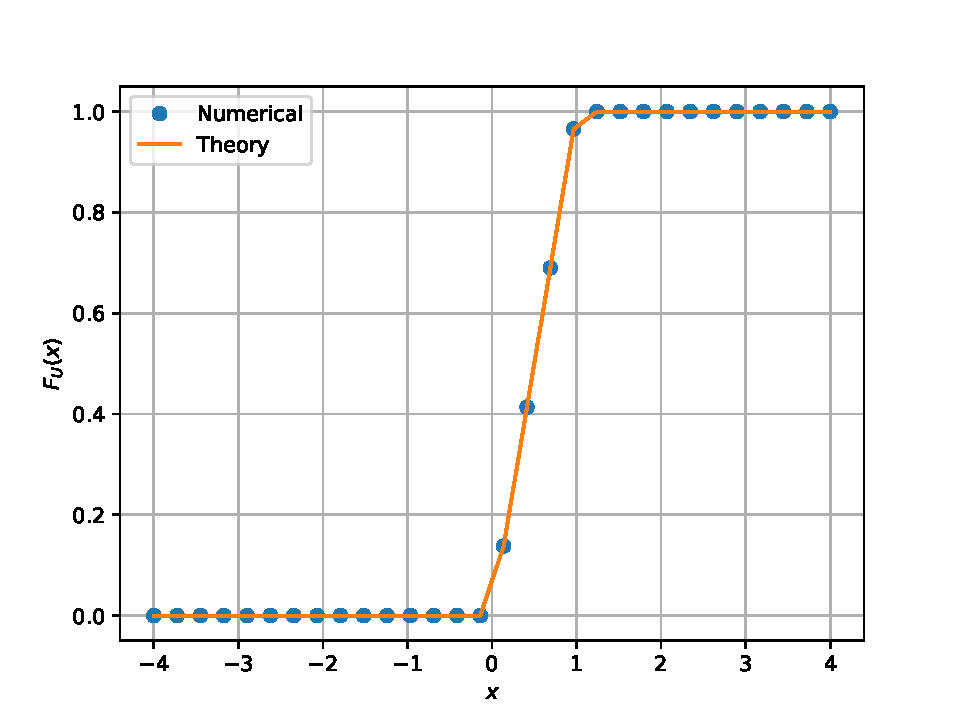
\includegraphics[width=\columnwidth]{Assignment-RandomNum/Figures/uni_cdf.pdf}
\caption{The CDF of $U$}
\label{fig:uni_cdf}
\end{figure}

\item Find a theoretical expression for $F_U\brak{x}$\\
\solution
Given, U is a uniform random variable. Let
\begin{align}
     p_U(x) &= 1 \text{ if x } \in \sbrak{0,1}
     \\
     F_U\brak{x} &= \pr{U \le x} 
     \\
     &= \int^{x}_{-\infty}p_U(x)dx
     \\
     &=
     \begin{cases}
        0, & x \in (-\infty,0) \\
        \int^{x}_{0}dx, & x \in [0,1]\\
        1, & x \in (1,\infty)
    \end{cases}
	\\	\therefore F_U\brak{x} &=
	\begin{cases}
        0, & x \in (-\infty,0) \\
        x, & x \in [0,1]\\
        1, & x \in (1,\infty)
    \end{cases}
	\label{eq:eq-1.3.1}
\end{align}
\item
The mean of $U$ is defined as
%
\begin{align}
	E\sbrak{U} = \frac{1}{N}\sum_{i=1}^{N}U_i
\end{align}
%
and its variance as
%
\begin{align}
\text{var}\sbrak{U} = E\sbrak{U- E\sbrak{U}}^2 
\end{align}
Write a C program to  find the mean and variance of $U$.\\
\solution 
Mean: 0.50007 Variance: 0.083301\\
Download the following files 
\begin{lstlisting}
wget https://github.com/Karthik-Kotikalapudi/AI1110/blob/main/Assignment-RandomNum/Codes/1.4.c
\end{lstlisting}
then compile and execute the C program using
\begin{lstlisting}
gcc 1.4.c -lm
./a.out
\end{lstlisting}
\item Verify your result theoretically given that
\end{enumerate}
%
\begin{align}
	E\sbrak{U^k} = \int_{-\infty}^{\infty}x^kdF_{U}(x)
	\label{eq:eq-1.5.1}
\end{align}
\solution Substituting $k=1$ in the equation \eqref{eq:eq-1.5.1}, and $F_U\brak{x}$ from equation \eqref{eq:eq-1.3.1}
\begin{align}
	E\sbrak{U} &= \int_{-\infty}^{\infty}xdF_{U}(x)
	\\
	E\sbrak{U} &= \int_{0}^{1}xdx
	\\
	\implies E\sbrak{U} &= \frac{1}{2}
	\\
	E\sbrak{U^2} &= \int_{0}^{1}x^2dx
	\\
	\implies E\sbrak{U^2} &= \frac{1}{3}
	\\
	Var\sbrak{U} &= E\sbrak{U^2} - \brak{E\sbrak{U}}^2
	\\
	\implies Var\sbrak{U} &= \frac{1}{6}
\end{align}

\section{Central Limit Theorem}
%
\begin{enumerate}[label=\thesection.\arabic*
,ref=\thesection.\theenumi]
%
\item
Generate $10^6$ samples of the random variable
%
\begin{equation}
X = \sum_{i=1}^{12}U_i -6
\end{equation}
%
using a C program, where $U_i, i = 1,2,\dots, 12$ are  a set of independent uniform random variables between 0 and 1
and save in a file called gau.dat\\
\solution 
Download the following file
\begin{lstlisting}
wget https://github.com/Karthik-Kotikalapudi/AI1110/blob/main/Assignment-RandomNum/Codes/2.1.c
\end{lstlisting}
\begin{lstlisting}
gcc 2.1.c
./a.out
\end{lstlisting}

\item Load gau.dat in python and plot the empirical CDF of $X$ using the samples in gau.dat. What properties does a CDF have?
\\
\solution 
We know that,
\begin{align}
Q(x) &= \pr{X>x}
\\
F_X(x) &= 1 - Q(x)
\end{align}
The CDF of $X$ is plotted in Fig. \ref{fig:gauss_cdf}
\begin{lstlisting}
wget https://github.com/Karthik-Kotikalapudi/AI1110/blob/main/Assignment-RandomNum/Codes/2.2.py
\end{lstlisting}
\begin{lstlisting}
$ python3 2.2.py
\end{lstlisting}
\begin{figure}[ht!]
\centering
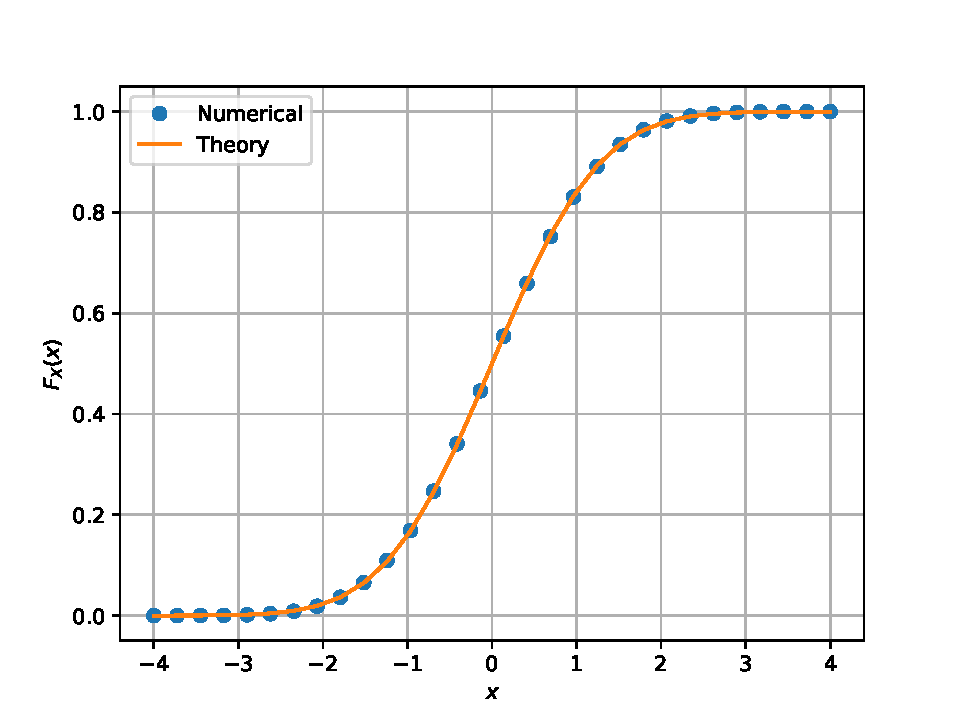
\includegraphics[width=\columnwidth]{Assignment-RandomNum/Figures/gau_cdf.pdf}
\caption{The CDF of $X$}
\label{fig:gauss_cdf}
\end{figure}
The properties of CDF are:
\begin{enumerate}
\item Monotonic Increasing function.
\item
\begin{align}
\lim_{x \to -\infty} F(x) = 0\\
\lim_{x \to \infty} F(x) = 1
\end{align}
\end{enumerate}

\item
Load gau.dat in python and plot the empirical PDF of $X$ using the samples in gau.dat. The PDF of $X$ is defined as
\begin{align}
p_{X}(x) = \frac{d}{dx}F_{X}(x)
\end{align}
What properties does the PDF have?
\\
\solution The PDF of $X$ is plotted in Fig. \ref{fig:gauss_pdf} using the code below
\begin{lstlisting}
wget https://github.com/Karthik-Kotikalapudi/AI1110/blob/main/Assignment-RandomNum/Codes/2.3.py
\end{lstlisting}
\begin{lstlisting}
$ python3 2.2.py
\end{lstlisting}
\begin{figure}[ht!]
\centering
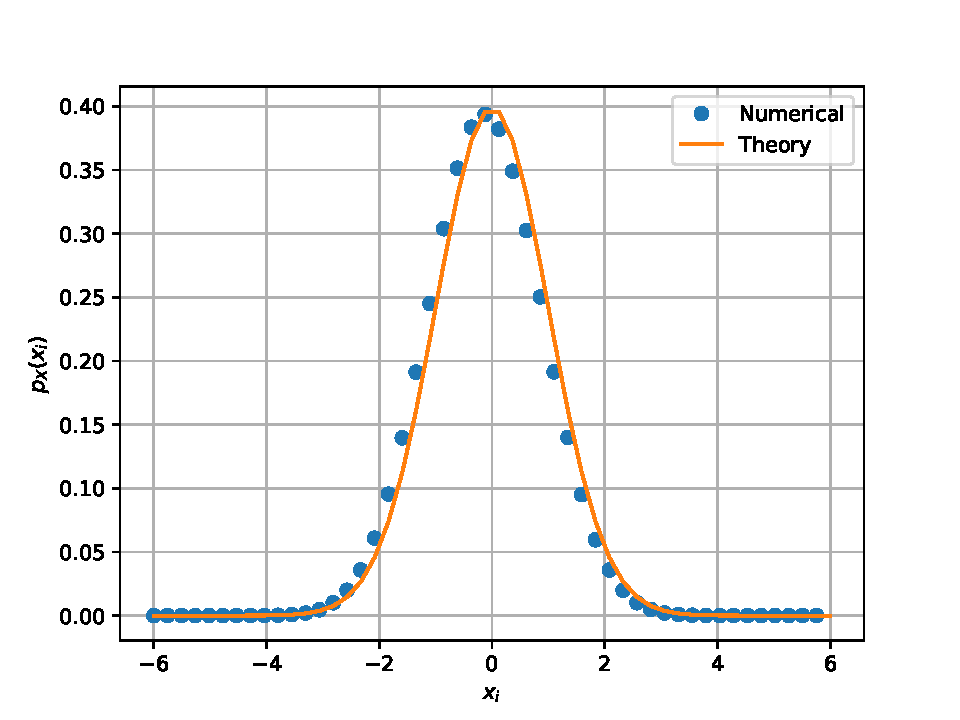
\includegraphics[width=\columnwidth]{Assignment-RandomNum/Figures/gau_pdf.pdf}
\caption{The PDF of $X$}
\label{fig:gauss_pdf}
\end{figure}
The properties of PDF are:
\begin{enumerate}
\item 
\begin{align}
\int_{-\infty}^{\infty}p(x)dx = 1
\end{align}
\item
$\forall x\in \mathbb{R} p(x) \ge 0$
\end{enumerate}

\item Find the mean and variance of $X$ by writing a C program.
\\
\solution 
Mean: 0.000294, variance: 0.999561
Download codes from
\begin{lstlisting}
wget https://github.com/Karthik-Kotikalapudi/AI1110/blob/main/Assignment-RandomNum/Codes/2.4.c
\end{lstlisting}
then compile and execute using
\begin{lstlisting}
gcc 2.4.c
./a.out
\end{lstlisting}
\item Given that 
\begin{align}
p_{X}(x) = \frac{1}{\sqrt{2\pi}}\exp\brak{-\frac{x^2}{2}}, -\infty < x < \infty,
\end{align}
repeat the above exercise theoretically.
\solution
From equation \eqref{eq:eq-1.5.1},
\begin{align}
	E\sbrak{X} &= \int^{\infty}_{-\infty}xp_x\brak{x}dx
	\\
	E\sbrak{X} &= \frac{1}{\sqrt{2\pi}}\int^{\infty}_{-\infty}xe^{\frac{-x^2}{2}}dx
\end{align}
Here $xe^{\frac{-x^2}{2}}$ is an odd function. Therefore,
\begin{align}
	E\sbrak{X} &= 0
\end{align}
\begin{align}
	Var\sbrak{X} &= \int^{\infty}_{-\infty}x^2p_x\brak{x}dx
	\\
	Var\sbrak{X} &= \frac{1}{\sqrt{2\pi}}\int^{\infty}_{-\infty}x^2e^{\frac{-x^2}{2}}dx
	\\
	\int x^2e^{\frac{-x^2}{2}} &= -xe^{\frac{-x^2}{2}}+\int e^{\frac{-x^2}{2}}dx
	\\
	\implies Var\sbrak{x} &= \frac{1}{\sqrt{2\pi}}\int^{\infty}_{-\infty}e^{\frac{-x^2}{2}}dx
	\\
	\implies Var\sbrak{x} &= \frac{\sqrt{2\pi}}{\sqrt{2\pi}}
\end{align}
\end{enumerate}

\section{From Uniform to Other}
\begin{enumerate}[label=\thesection.\arabic*
,ref=\thesection.\theenumi]
\item
Generate samples of 
%
\begin{align}
V = -2\ln\brak{1-U}
\end{align}
%
and plot its CDF.\\
\solution
Download the files from
\begin{lstlisting}
wget https://github.com/Karthik-Kotikalapudi/AI1110/blob/main/Assignment-RandomNum/Codes/3.1.c
wget https://github.com/Karthik-Kotikalapudi/AI1110/blob/main/Assignment-RandomNum/Codes/3.1.py
\end{lstlisting}
then compile and execute the  C program then run the python program using
\begin{lstlisting}
gcc 3.1.c
./a.out
python3 3.1.py
\end{lstlisting}
The CDF of $V$ is plotted in Fig. \ref{fig:v_cdf}
\begin{figure}[ht!]
\centering
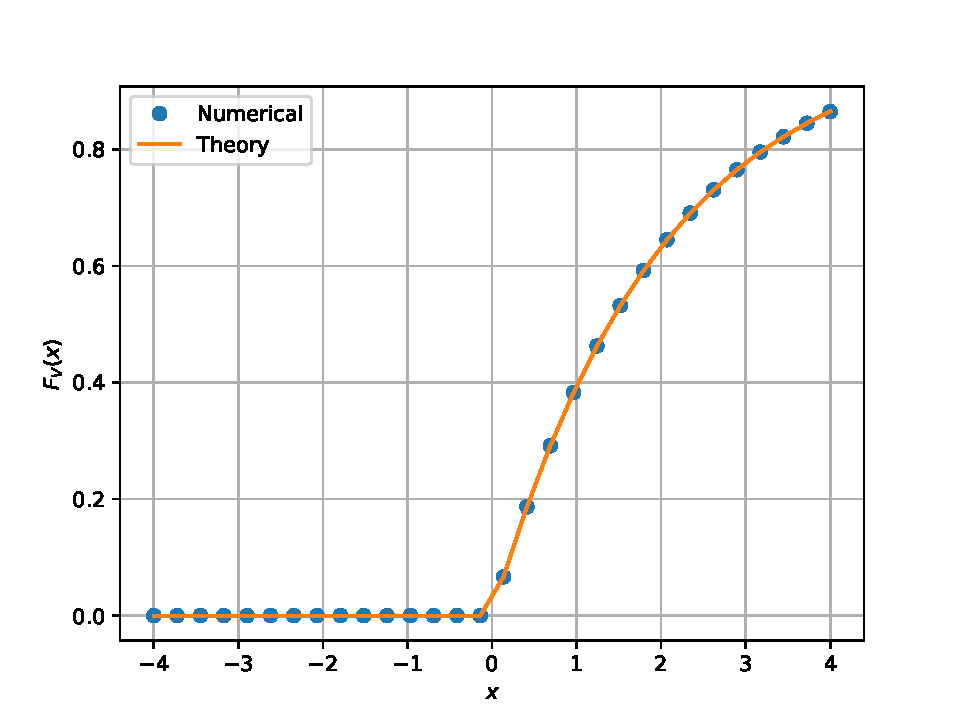
\includegraphics[width=\columnwidth]{Assignment-RandomNum/Figures/v_cdf.pdf}
\caption{The CDF of $V$}
\label{fig:v_cdf}
\end{figure}

\item Find a theoretical expression for $F_V(x)$.\\
\solution
We know that
\begin{align}
	F_V\brak{v} &= \pr{V\le v}
	\label{eq:eq-3.2.1}
	\\
	V &= -2\ln\brak{1-U}
	\label{eq:eq-3.2.2}
\end{align}
Substituting equation \eqref{eq:eq-3.2.2} in equation \eqref{eq:eq-3.2.1},
\begin{align}
	F_V\brak{x} &= \pr{-2\ln\brak{1-U}\le x}
	\\
	&= \pr{U\le 1-e^{-\frac{x}{2}}}
	\\
	&= F_U\brak{1-e^{-\frac{x}{2}}}
\end{align}
From equation \eqref{eq:eq-1.3.1}, 
\begin{align}
	F_V\brak{x} = 1- e^{-\frac{x}{2}}
\end{align}

\end{enumerate}
\section{Triangular Distribution}
\begin{enumerate}[label=\thesection.\arabic*
,ref=\thesection.\theenumi]
%
\item Generate 
	\begin{align}
		T = U_1+U_2
	\end{align}
\solution 
Download the files from
\begin{lstlisting}
wget https://github.com/Karthik-Kotikalapudi/AI1110/blob/main/Assignment-RandomNum/Codes/4.1.c
\end{lstlisting}
then compile and execute the  C program using
\begin{lstlisting}
gcc 4.1.c
./a.out
\end{lstlisting}
\item Find the CDF of $T$.\\
\solution
The CDF of T is plotted in the Fig. \ref{fig:tri_cdf}\\
Download the files from
\begin{lstlisting}
wget https://github.com/Karthik-Kotikalapudi/AI1110/blob/main/Assignment-RandomNum/Codes/4.2.py
\end{lstlisting}
then run the python program using
\begin{lstlisting}
python3 4.2.py
\end{lstlisting}
\begin{figure}[ht!]
\centering
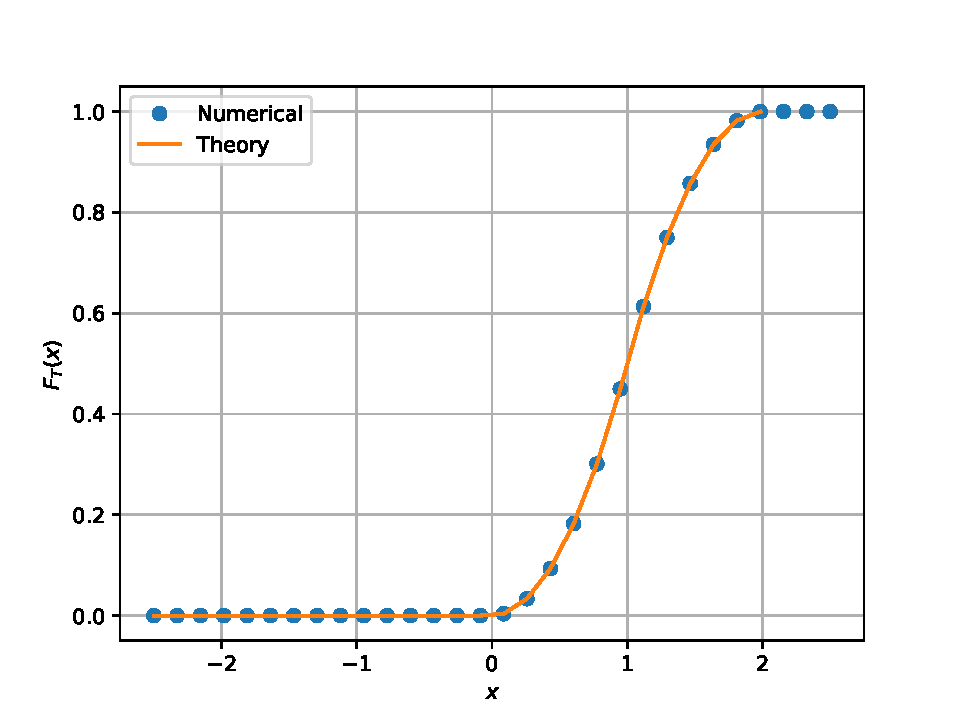
\includegraphics[width=\columnwidth]{Assignment-RandomNum/Figures/tri_cdf.pdf}
\caption{The CDF of $T$}
\label{fig:tri_cdf}
\end{figure}
\item Find the PDF of $T$.
\solution
The CDF of T is plotted in the Fig. \ref{fig:tri_pdf}\\
Download the files from
\begin{lstlisting}
wget https://github.com/Karthik-Kotikalapudi/AI1110/blob/main/Assignment-RandomNum/Codes/4.3.py
\end{lstlisting}
then run the python program using
\begin{lstlisting}
python3 4.3.py
\end{lstlisting}
\begin{figure}[ht!]
\centering
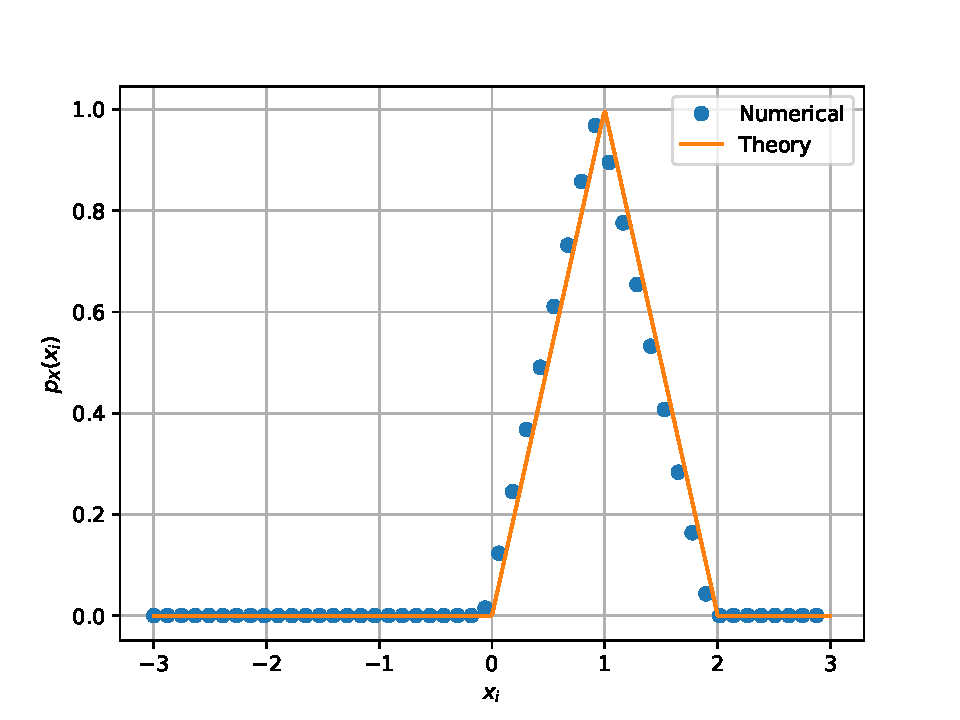
\includegraphics[width=\columnwidth]{Assignment-RandomNum/Figures/tri_pdf.pdf}
\caption{The PDF of $T$}
\label{fig:tri_pdf}
\end{figure}
\item Find the theoretical expressions for the PDF and CDF of $T$.\\
\solution
For calculating PDF, we know that
\begin{align}
	T &= U_1+U_2
	\\
	f_T(t) &= \int^{\infty}_{-\infty}f_{U_1}(u)f_{U_2}(t-u)dt
	\\
	f_T(t) &= \int^{2}_{0}f_{U_1}(u)f_{U_2}(t-u)dt
\end{align}
If $0<t<1$,
\begin{align}
	f_T(t) &= \int^{1}_{0}f_{U_2}(t-u)dt
	\\
	f_T(t) &= \int^{t}_{0}f_{U_2}(t-u)dt
	\\
	f_T(t) &= t
\end{align}
If $1<t<2$,
\begin{align}
	f_T(t) &= \int^{2}_{1}f_{U_2}(t-u)dt
	\\
	f_T(t) &= \int^{t}_{1}f_{U_2}(t-u)dt
	\\
	f_T(t) &= 2-t
\end{align}
For CDF,
\begin{align}
    F_T(x) &= \int _{-\infty} ^x p_T(t) dt
    \\
    F_T(x) &= 
    \begin{cases}
        0, & x \in (-\infty,0) \\
        \frac{x^2}{2}, & x \in (0,1) \\
        -\frac{x^2}{2} + 2x - 1, & x \in (1, 2) \\
        1, & x \in (2,\infty)
    \end{cases}
\end{align}

\item Verify your results through a plot.\\
\solution
The theoritical CDF and PDF of $T$ are plotted in the Figures, Fig. \ref{fig:tri_cdf}, Fig. \ref{fig:tri_pdf} respectively.
\end{enumerate}
\section{Maximul Likelihood}
\begin{enumerate}[label=\thesection.\arabic*
,ref=\thesection.\theenumi]
\item Generate 
\begin{equation}
Y = AX+N,
\end{equation}
where $A = 5 \text{ dB}, X \in \cbrak{1,-1}$,  is Bernoulli and $N \sim \mathcal{N}\brak{0,1}$.
	\item Plot $Y$.
	\item Guess how to estimate $X$ from $Y$.
\item
\label{ml-ch4_sim}
Find 
\begin{equation}
	P_{e|0} = \pr{\hat{X} = -1|X=1}
\end{equation}
and 
\begin{equation}
	P_{e|1} = \pr{\hat{X} = 1|X=-1}
\end{equation}
%
\item Find $P_e$.
%
\item
Verify by plotting  the theoretical $P_e$.  
		\end{enumerate}
\section{Gaussian to Other}
\begin{enumerate}[label=\thesection.\arabic*
,ref=\thesection.\theenumi]
\item
Let $X_1 \sim  \mathcal{N}\brak{0,1}$ and $X_2 \sim  \mathcal{N}\brak{0,1}$. Plot the CDF and PDF of
%
\begin{equation}
V = X_1^2 + X_2^2
\end{equation}
%
%
%
\item
If
%
\begin{equation}
F_{V}(x) = 
\begin{cases}
1 - e^{-\alpha x} & x \geq 0 \\
0 & x < 0,
\end{cases}
\end{equation}
%
find $\alpha$.
%
\item
\label{ch3_raleigh_sim}
Plot the CDF and PDf of
%
\begin{equation}
A = \sqrt{V}
\end{equation}
%
\end{enumerate}
\end{document}